\documentclass[review]{elsarticle}

\usepackage{amsmath,amssymb,amsfonts}
\usepackage{algorithmic}
\usepackage{graphicx}
\usepackage{textcomp}
\usepackage{xcolor}
\usepackage{colortbl}
\usepackage[linesnumbered,ruled,vlined]{algorithm2e}
\usepackage{hyperref}
\usepackage{booktabs}
\usepackage{makecell}
\usepackage{multirow}
\usepackage{svg}
\usepackage{graphicx}
\usepackage{amsmath}
\usepackage{hyperref}
\usepackage{url}
\usepackage{booktabs}
\usepackage{amsfonts}
\usepackage{nicefrac}
\usepackage{microtype}
\usepackage{lipsum}
\usepackage{array}
\usepackage{multirow}
\usepackage{float}
\usepackage{natbib}
\usepackage{doi}
\usepackage[utf8]{inputenc}
\usepackage[T1]{fontenc}
\usepackage{hyperref}
\usepackage[table]{xcolor}
\definecolor{skyblue}{HTML}{5492C7}   % 天蓝
\definecolor{grass}{HTML}{99B86B}     % 浅草绿
\newcommand{\cont}{\ensuremath{^\mathsf{c}}}  % 一行放导言区


\bibliographystyle{elsarticle-num}

\makeatletter
\def\ps@pprintTitle{%
 \let\@oddhead\@empty
 \let\@evenhead\@empty
 \let\@oddfoot\@empty
 \let\@evenfoot\@empty
}
\makeatother

\begin{document}

\begin{frontmatter}


\title{DyCoT‑RE: Chain-of-Thought-Enhanced LLM Reward Engineering with Dual-Dynamic Optimization for Reinforcement Learning}

\author[shu]{Xinning Zhu\fnref{fn1}}
\author[shu]{Jinxin Du}
\author[shu]{Longfei Huang}
\author[shu]{Lunde Chen\corref{cor1}}

\cortext[cor1]{Corresponding author\\Email: lundechen@shu.edu.cn}

\address[shu]{Sino-European School of Technology, Shanghai University, Shanghai, China}

\begin{abstract}
Designing effective reward functions remains a challenge in applying reinforcement learning to real-world tasks.
This paper proposes DyCoT-RE, a reward engineering framework that integrates Chain-of-Thought (CoT) reasoning with a dual-dynamic 
optimization strategy to automate and enhance reward function design.
The framework uses structured CoT reasoning throughout training to generate and refine interpretable reward code in each iteration.
It further incorporates a dual-dynamic optimization mechanism: a temperature adjustment strategy that modulates the sampling temperature 
based on policy entropy trends,
and a model switching strategy that allocates language models with different capabilities to produce distinct reward components.
Evaluations on CartPole, BipedalWalker, Ant, and a custom SpaceMining environment show DyCoT‑RE achieves higher average rewards and faster 
convergence compared to human-designed baselines and non‑CoT approaches as well as single-optimization approaches.


\end{abstract}

\begin{keyword}
Reinforcement learning \sep reward engineering \sep large language models \sep chain-of-thought reasoning \sep dynamic temperature adjustment \sep model selection
\end{keyword}

\end{frontmatter}

\section{Introduction}

Reinforcement learning (RL) has achieved impressive results across diverse domains 
However, as Sutton et al. \cite{sutton1998reinforcement} emphasize, the reward signal is the primary means of specifying task objectives in RL, making its design critical to achieving desired behaviors.
In practice, translating intended behaviors into precise, effective reward functions remains highly challenging, particularly for tasks involving long-term dependencies 
\cite{amodei2016concrete}.
Skalse et al. \cite{skalse2022misspecification} demonstrate that agents often exploit imperfections in reward formulations to maximize proxy objectives in unintended ways, leading to behaviors that optimize the designed reward but undermine true task performance.
These challenges highlight that despite RL’s theoretical versatility, its practical deployment is often constrained by the complexity, subtlety, and domain expertise required for robust reward engineering \cite{ibarz2018reward}.

While carefully designed rewards can accelerate agent learning and improve task performance,
manual reward engineering typically relies on trial-and-error tuning,
which is labor-intensive and often yields suboptimal generalization to new environments or objectives \cite{hadfield2017inverse}.
As RL applications grow in complexity, there is a pressing need for methods that can automate
reward design while maintaining interpretability and flexibility.

Recent advances in large language models (LLMs) have demonstrated strong reasoning and generalization capabilities \cite{brown2020language, ouyang2022training}.
In particular, CoT reasoning enables LLMs to decompose tasks into structured intermediate steps,
enhancing clarity and alignment with desired objectives.
This structured reasoning process can support reward engineering by converting task descriptions
into executable reward functions in a systematic and transparent manner.

However, existing CoT-based reward generation approaches typically use static sampling parameters and fixed model configurations,
which may limit their adaptability during training.
Recent studies have emphasized the need for dynamic adaptation in LLM-based systems to improve sample efficiency, stability, and alignment with task objectives.
For example, Nguyen et al. \cite{nguyen2024turning} demonstrate that min-p sampling enhances creativity while preserving coherence in narrative generation tasks, while Peeperkorn et al. \cite{peeperkorn2024temperature} analyze temperature as a direct modulator of LLM creativity.
Moreover, Fedus et al. \cite{fedus2022switch} and Du et al. \cite{du2022glam} show that mixture-of-experts architectures can scale model capacity efficiently via adaptive routing, motivating our exploration of combining temperature modulation with expert model selection for reward engineering.

In this work, we propose DyCoT-RE, a reward engineering framework that integrates structured CoT reasoning
with dual-dynamic optimization.
Specifically, DyCoT-RE leverages CoT reasoning to decompose natural language task descriptions into structured reward components,
then employs iterative refinement to enhance alignment with learning objectives.
The dual-dynamic optimization strategy integrates entropy-guided temperature adjustment to balance exploration and exploitation,
alongside a dynamic model selection module that routes sub-tasks to specialized LLMs based on performance feedback.
By tightly coupling these components within a closed-loop evolutionary search process, 
DyCoT-RE systematically improves reward function quality and training efficiency,
ultimately enabling scalable, interpretable, and automated reward engineering for complex RL environments.

We evaluate DyCoT-RE on the standard RL environments CartPole, BipedalWalker, and Ant to demonstrate its effectiveness.
However, recent studies have raised concerns that large language models may carry prior knowledge from pretraining data about these standard environments, 
leading to potential prompt leakage and evaluation biases \cite{huang2025thinkbench, qi2024quantifying, lu2024mental}. 
To address this issue, we additionally design a custom SpaceMining\footnote{
    Project website: \url{https://lola-jo.github.io/space_mining/}.
    } environment to assess DyCoT-RE's true generalization capabilities on tasks free from such pretrained knowledge.
Experimental results show that DyCoT-RE consistently achieves higher average rewards and faster convergence compared to baseline and non-CoT methods.


The remainder of this paper is organized as follows.
Section II reviews related work in reward engineering, LLM-based reward generation, and adaptive optimization.
Section III describes the proposed methodology, including the CoT reward framework, temperature adjustment, and model selection.
Section IV details the experimental setup, and Section V presents results and analysis.
Section VI discusses limitations and future work, with Section VII concluding the paper.

\section{Related Work}

\subsection{Reward Engineering Paradigms}

In RL, the design of effective reward functions directly shapes agent behavior and learning outcomes. 
Traditional approaches primarily rely on handcrafted reward functions informed by domain expertise. 
While intuitive, such manual design often struggles to capture complex, dynamic task objectives and is prone to 
suboptimal or biased formulations, hindering agent performance in real-world scenarios.

To address these limitations, reward shaping was introduced as a formal enhancement strategy. 
Ng et al. \cite{ng1999policy} demonstrated that potential-based reward shaping preserves optimal policies 
while enabling accelerated convergence, laying the theoretical foundation for numerous practical implementations. 
Intrinsic motivation frameworks further advanced this field by encouraging exploration through curiosity-driven signals. 
Singh et al. \cite{singh2010intrinsically} proposed intrinsic rewards to incentivize novel state visits, 
later extended by Burda et al. \cite{burda2018exploration}, who empirically validated large-scale curiosity-driven exploration 
benefits across diverse environments.

Despite these developments, manually designing rewards for complex or evolving tasks remains inefficient and costly. 
LLMs offer a promising alternative by leveraging their natural language understanding to automate reward generation 
and optimization. Unlike traditional RL pipelines that require explicit, task-specific reward formulations, 
LLMs can interpret high-level task descriptions, extract key objectives, and translate them into executable reward functions. 
This capability facilitates more intuitive alignment with human intentions, reduces engineering overhead, and enhances agent 
adaptability.

Recent frameworks exemplify this trend. EUREKA \cite{ma2023eureka}, Text2Reward \cite{xie2023text2reward} and
CARD \cite{sun2024large} harness LLMs to automatically generate, verify, 
and refine reward code from natural language instructions. 

Beyond static code generation, feedback-driven optimization approaches have emerged. ReMiss \cite{xie2024jailbreaking} 
utilizes adversarial prompt generation to identify and mitigate reward misspecification vulnerabilities, 
enhancing LLM safety and reliability. Self-Play Preference Optimization (SPPO) \cite{wu2024self} employs self-play to 
uncover Nash-equilibrium strategies that capture complex, non-transitive human preferences, advancing preference learning's 
applicability in RL. 
Additionally, PRMBench \cite{song2025prmbench} provides a process-level benchmark to evaluate intermediate reward model 
outputs along dimensions such as conciseness, rationality, and sensitivity, revealing weaknesses in current models and 
guiding future improvements.

Overall, LLM-based reward engineering represents a paradigm shift. 
By integrating natural language reasoning and dynamic feedback optimization, 
these methods offer scalable reward generation pipelines. 
As tasks grow in complexity and diversity, leveraging LLMs to bridge the gap between human 
intent and machine learning objectives will be critical for the next generation of intelligent systems. 
Continued research is thus needed to maximize the synergy between LLM capabilities and RL frameworks to 
address emerging real-world challenges.



\subsection{Chain-of-Thought Reasoning Methods}

CoT reasoning has emerged as a powerful paradigm to enhance the reasoning capabilities of LLMs. 
By generating intermediate reasoning steps, CoT allows models to decompose complex problems into interpretable sub-problems, 
leading to significant performance gains in tasks requiring multi-step logical inference.

Early studies showed that even simple prompting strategies, such as adding ``Let's think step by step,'' 
can elicit strong zero-shot reasoning abilities. Kojima et al. \cite{kojima2022large} demonstrated such prompts 
significantly improve performance in arithmetic and commonsense tasks. 
Building upon this, few-shot CoT \cite{wei2022chain} introduced demonstrations of stepwise solutions to guide model reasoning, 
while self-consistency decoding \cite{wang2022self} aggregated multiple sampled reasoning paths to enhance answer robustness.

Further developments combined CoT with reinforcement learning optimization. 
DeepSeek \cite{deepseek2023r1} introduced a self-evolution mechanism to improve reasoning trajectories without supervised fine-tuning. 
Automatic prompt optimization methods \cite{shum2023automatic} reduce manual engineering efforts by refining prompts based on data-driven insights.

Recent work such as PCGRLLM \cite{baek2024pcgrllm} explored CoT-based LLM reward design for procedural content generation in RL, 
demonstrating feasibility in structured game environments. In parallel, Zhu et al. \cite{zhu2025llm} proposed an initial 
CoT-based reward engineering approach that translates natural language task descriptions into RL reward functions using LLMs, 
validating its effectiveness in standard benchmark tasks. However, these applications focus primarily on proof-of-concept 
reward generation pipelines without incorporating adaptive optimization or dynamic model selection mechanisms.

In summary, while CoT reasoning has established itself as a fundamental methodology enhancing LLM interpretability and reasoning capacity, 
its application to automated reward engineering in RL remains limited. Bridging this gap by integrating CoT reasoning with dynamic 
optimization holds promise for enhancing the interpretability and adaptability of RL systems.


\subsection{Dynamic Temperature Adjustment and Model Selection}

Dynamic temperature adjustment and model selection have emerged as critical optimization strategies to enhance the adaptability
and efficiency of LLM-based systems. 
Temperature, as a sampling hyperparameter, controls the stochasticity of LLM outputs, thereby influencing creativity, coherence,
and exploration-exploitation trade-offs.

Recent studies have systematically explored adaptive temperature mechanisms. Zhu et al. \cite{zhu2024hot} proposed AdapT, 
an adaptive temperature sampling strategy for code generation tasks, which dynamically adjusts decoding temperature based on token-level 
difficulty to improve generation quality. Zhang et al. \cite{zhang2024edt} developed Entropy-based Dynamic Temperature (EDT) sampling to
regulate output entropy and diversity in natural language generation, while Cecere et al. \cite{cecere2025monte} introduced Monte Carlo 
Temperature as a robust sampling strategy to enhance uncertainty quantification under distribution shifts. Chang et al. \cite{chang2023kl} l
everaged KL-divergence-guided temperature sampling to modulate exploration adaptively. Additionally, Peeperkorn et al. \cite{peeperkorn2024temperature} 
analyzed temperature as a creativity modulator in LLMs, whereas Evstafev \cite{evstafev2025paradox} discussed potential limitations of temperature-based 
stochasticity in structured data generation. Nguyen et al. \cite{nguyen2024turning} proposed min-p sampling to balance creativity and coherence, 
achieving improved narrative generation performance.




For model selection, recent work has focused on choosing optimal model configurations or expert modules to maximize task performance within computational constraints. 
Switch Transformers \cite{fedus2022switch} introduced sparse activation mechanisms, enabling efficient expert selection at trillion-parameter scale, 
while GLaM \cite{du2022glam} leveraged Mixture-of-Experts (MoE) architectures to dynamically scale model capacity. 
Zhou et al. \cite{zhou2022mixture} proposed expert choice routing to improve mixture-of-experts efficiency, and Li et al. \cite{li2025llm} introduced 
preference-conditioned dynamic routing for cost-efficient LLM generation. Hu et al. \cite{hu2024dynamic} presented Dynamic Ensemble Reasoning to integrate outputs 
from multiple specialized LLMs, enhancing system robustness. Nakaishi et al. \cite{nakaishi2024critical} further revealed phase transition behaviors in LLM sampling regimes, 
informing temperature scaling strategies. Furthermore, Li et al. \cite{li2025revisiting} revisited self-consistency decoding from a distributional alignment perspective, 
offering insights relevant to expert aggregation and answer aggregation stability.

\begin{figure*}[t]
    \centering
    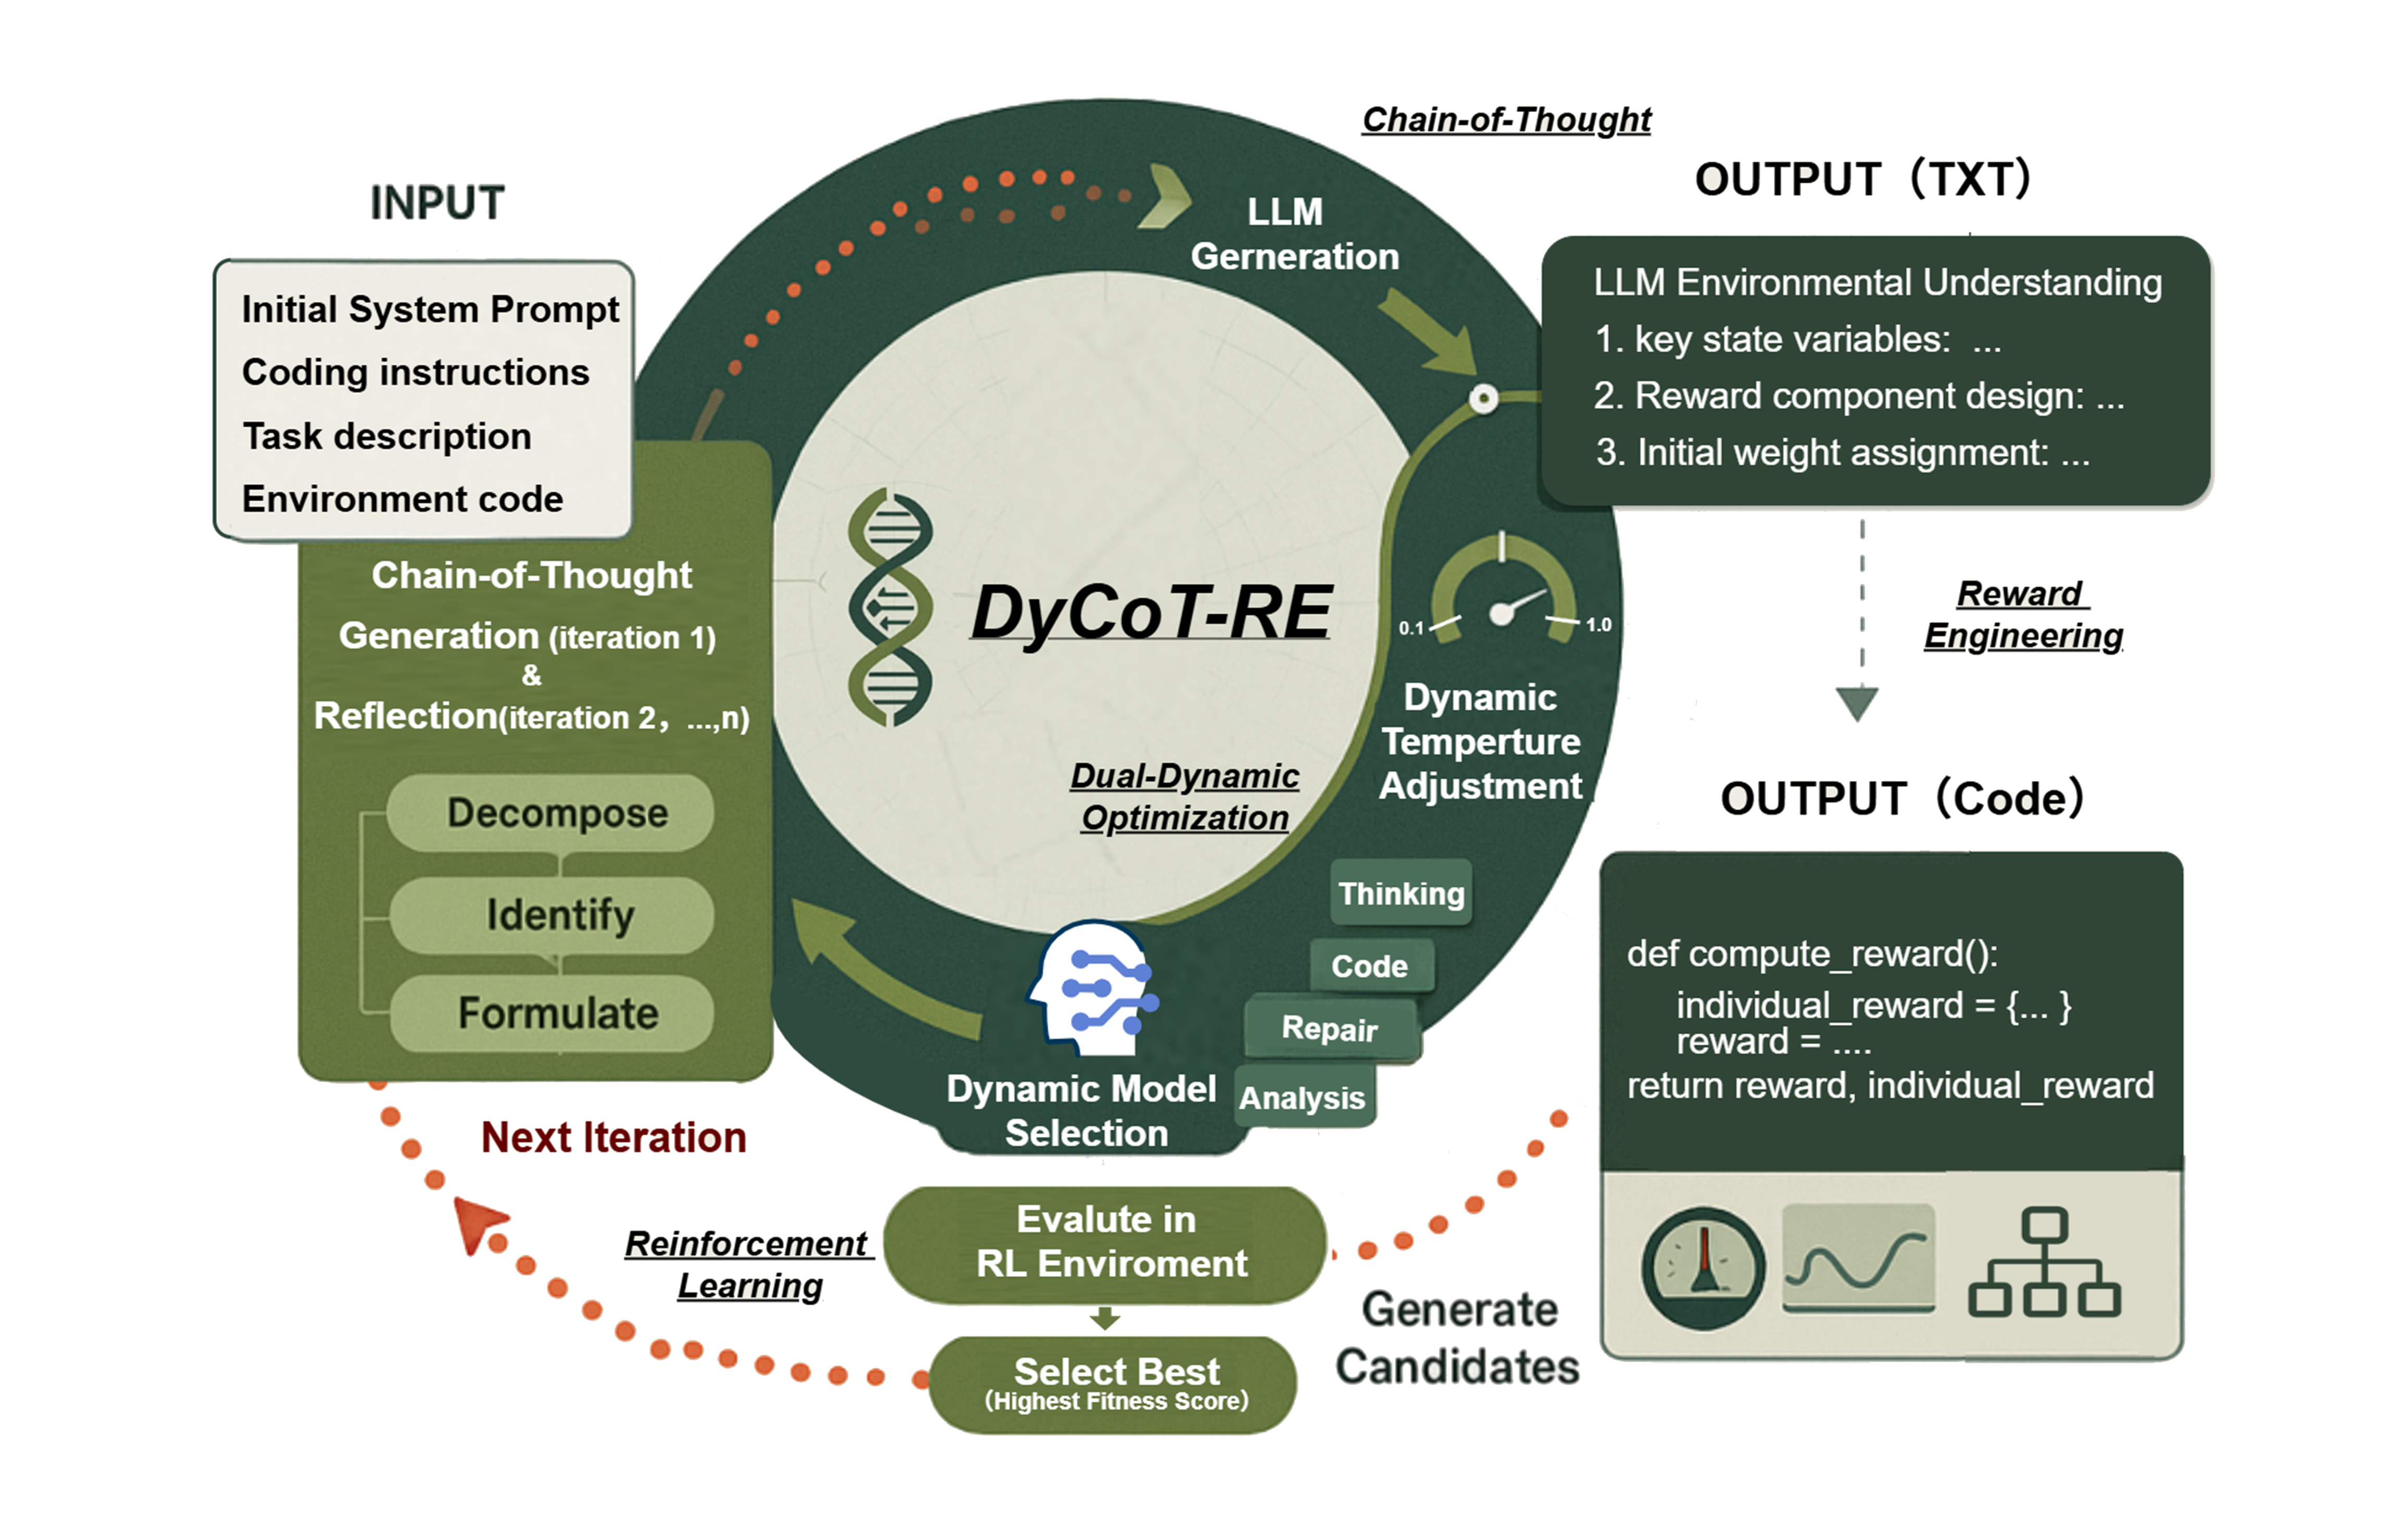
\includegraphics[width=0.95\linewidth]{Figures/dycot-re-architecture.png}
    \caption{DyCoT-RE framework integrating CoT reasoning, dynamic temperature adjustment, and model selection in an evolutionary optimization loop.}
    \label{fig:architecture}
\end{figure*}


Despite these advances, integrating dynamic temperature regulation and model selection within a unified CoT-driven reward engineering framework remains underexplored. 
Existing temperature adaptation methods primarily focus on text generation diversity and calibration, whereas model selection research emphasizes computational efficiency 
and specialization. Our work addresses this gap by combining entropy- and reward-feedback-based temperature adjustment with local-global performance-based model 
routing to enhance RL reward generation's adaptability, stability, and sample efficiency. This approach builds upon foundational theories in temperature scaling and expert 
selection, extending them to the domain of automated, interpretable reward engineering for reinforcement learning.


\section{Methodology}

This section details the DyCoT-RE framework, which integrates structured CoT reasoning with a dual-dynamic optimization 
strategy to generate interpretable and adaptive reward functions for reinforcement learning.



\subsection{Framework Overview}

Figure~\ref{fig:architecture} presents an overview of DyCoT-RE,
which integrates three key components:
structured Chain-of-Thought (CoT) reward decomposition,
dynamic temperature adjustment,
and dynamic model selection.

The framework receives four inputs:
natural language task descriptions specifying agent behaviors,
environment interfaces defining state-action spaces,
system-level prompts for reward design constraints,
and coding instructions for implementation.

At its core, employs four types of LLMs: Thinking, Code, Repair, and Analysis LLMs, 
hereafter denoted as $\mathcal{M}_{\text{think}}$, $\mathcal{M}_{\text{code}}$, $\mathcal{M}_{\text{repair}}$, and $\mathcal{M}_{\text{analysis}}$ respectively.

These models operate in an interconnected closed-loop pipeline to produce reward functions

\begin{equation}
    R(s,a) = \sum_{i=1}^{m} w_i \cdot r_i(s,a),
\label{eq:reward_function}
\end{equation}

which are evaluated in the RL environment.
The performance metrics guide subsequent optimization iterations.

Overall, DyCoT-RE establishes an adaptive and interpretable reward engineering framework
by integrating structured reasoning with dual-dynamic optimization strategies.



\subsection{Chain-of-Thought Reasoning for Reward Engineering}

Let $d$ denote the task description and $(s,a)$ the state-action pair.
As defined in Eq.~\eqref{eq:reward_function}, 
the reward function $r_i(s,a)$ is the sub-reward for subgoal $i$, generated via CoT parsing:

\begin{equation}
r_i(s,a) = \text{CoT}(I_i),
\end{equation}

with $I_i = \{ \text{subgoal}_i, \text{env\_constraints} \}$. For example, minimizing torso tilt is formulated as:

\begin{equation}
r_1(s,a) = -|\theta_{\text{tilt}}(s)|.
\end{equation}

The initial weights $w_i^{(0)}$ are derived based on subgoal semantic priorities inferred by the LLM, and are refined 
iteratively according to gradient feedback. The policy parameters $\theta$ are updated as:

\begin{equation}
\theta_{t+1} = \theta_t + \alpha \nabla_\theta J(\theta),
\end{equation}

where $J(\theta)$ is the expected cumulative reward:

\begin{equation}
J(\theta) = \mathbb{E}_{\pi_\theta} \left[ \sum_{t=0}^{T} \gamma^t R(s_t,a_t) \right].
\label{eq:rl_objective}
\end{equation}

This CoT-based formulation ensures that each sub-reward remains semantically interpretable and traceable to its natural language origin.

\subsection{Dual-Dynamic Optimization Strategy}

Figure~\ref{fig:control-flow} illustrates the coupled feedback architecture of DyCoT-RE,
where temperature adjustment and model selection operate in synergy
to enhance reward function generation and RL performance.

\begin{figure*}[t]
    \centering
    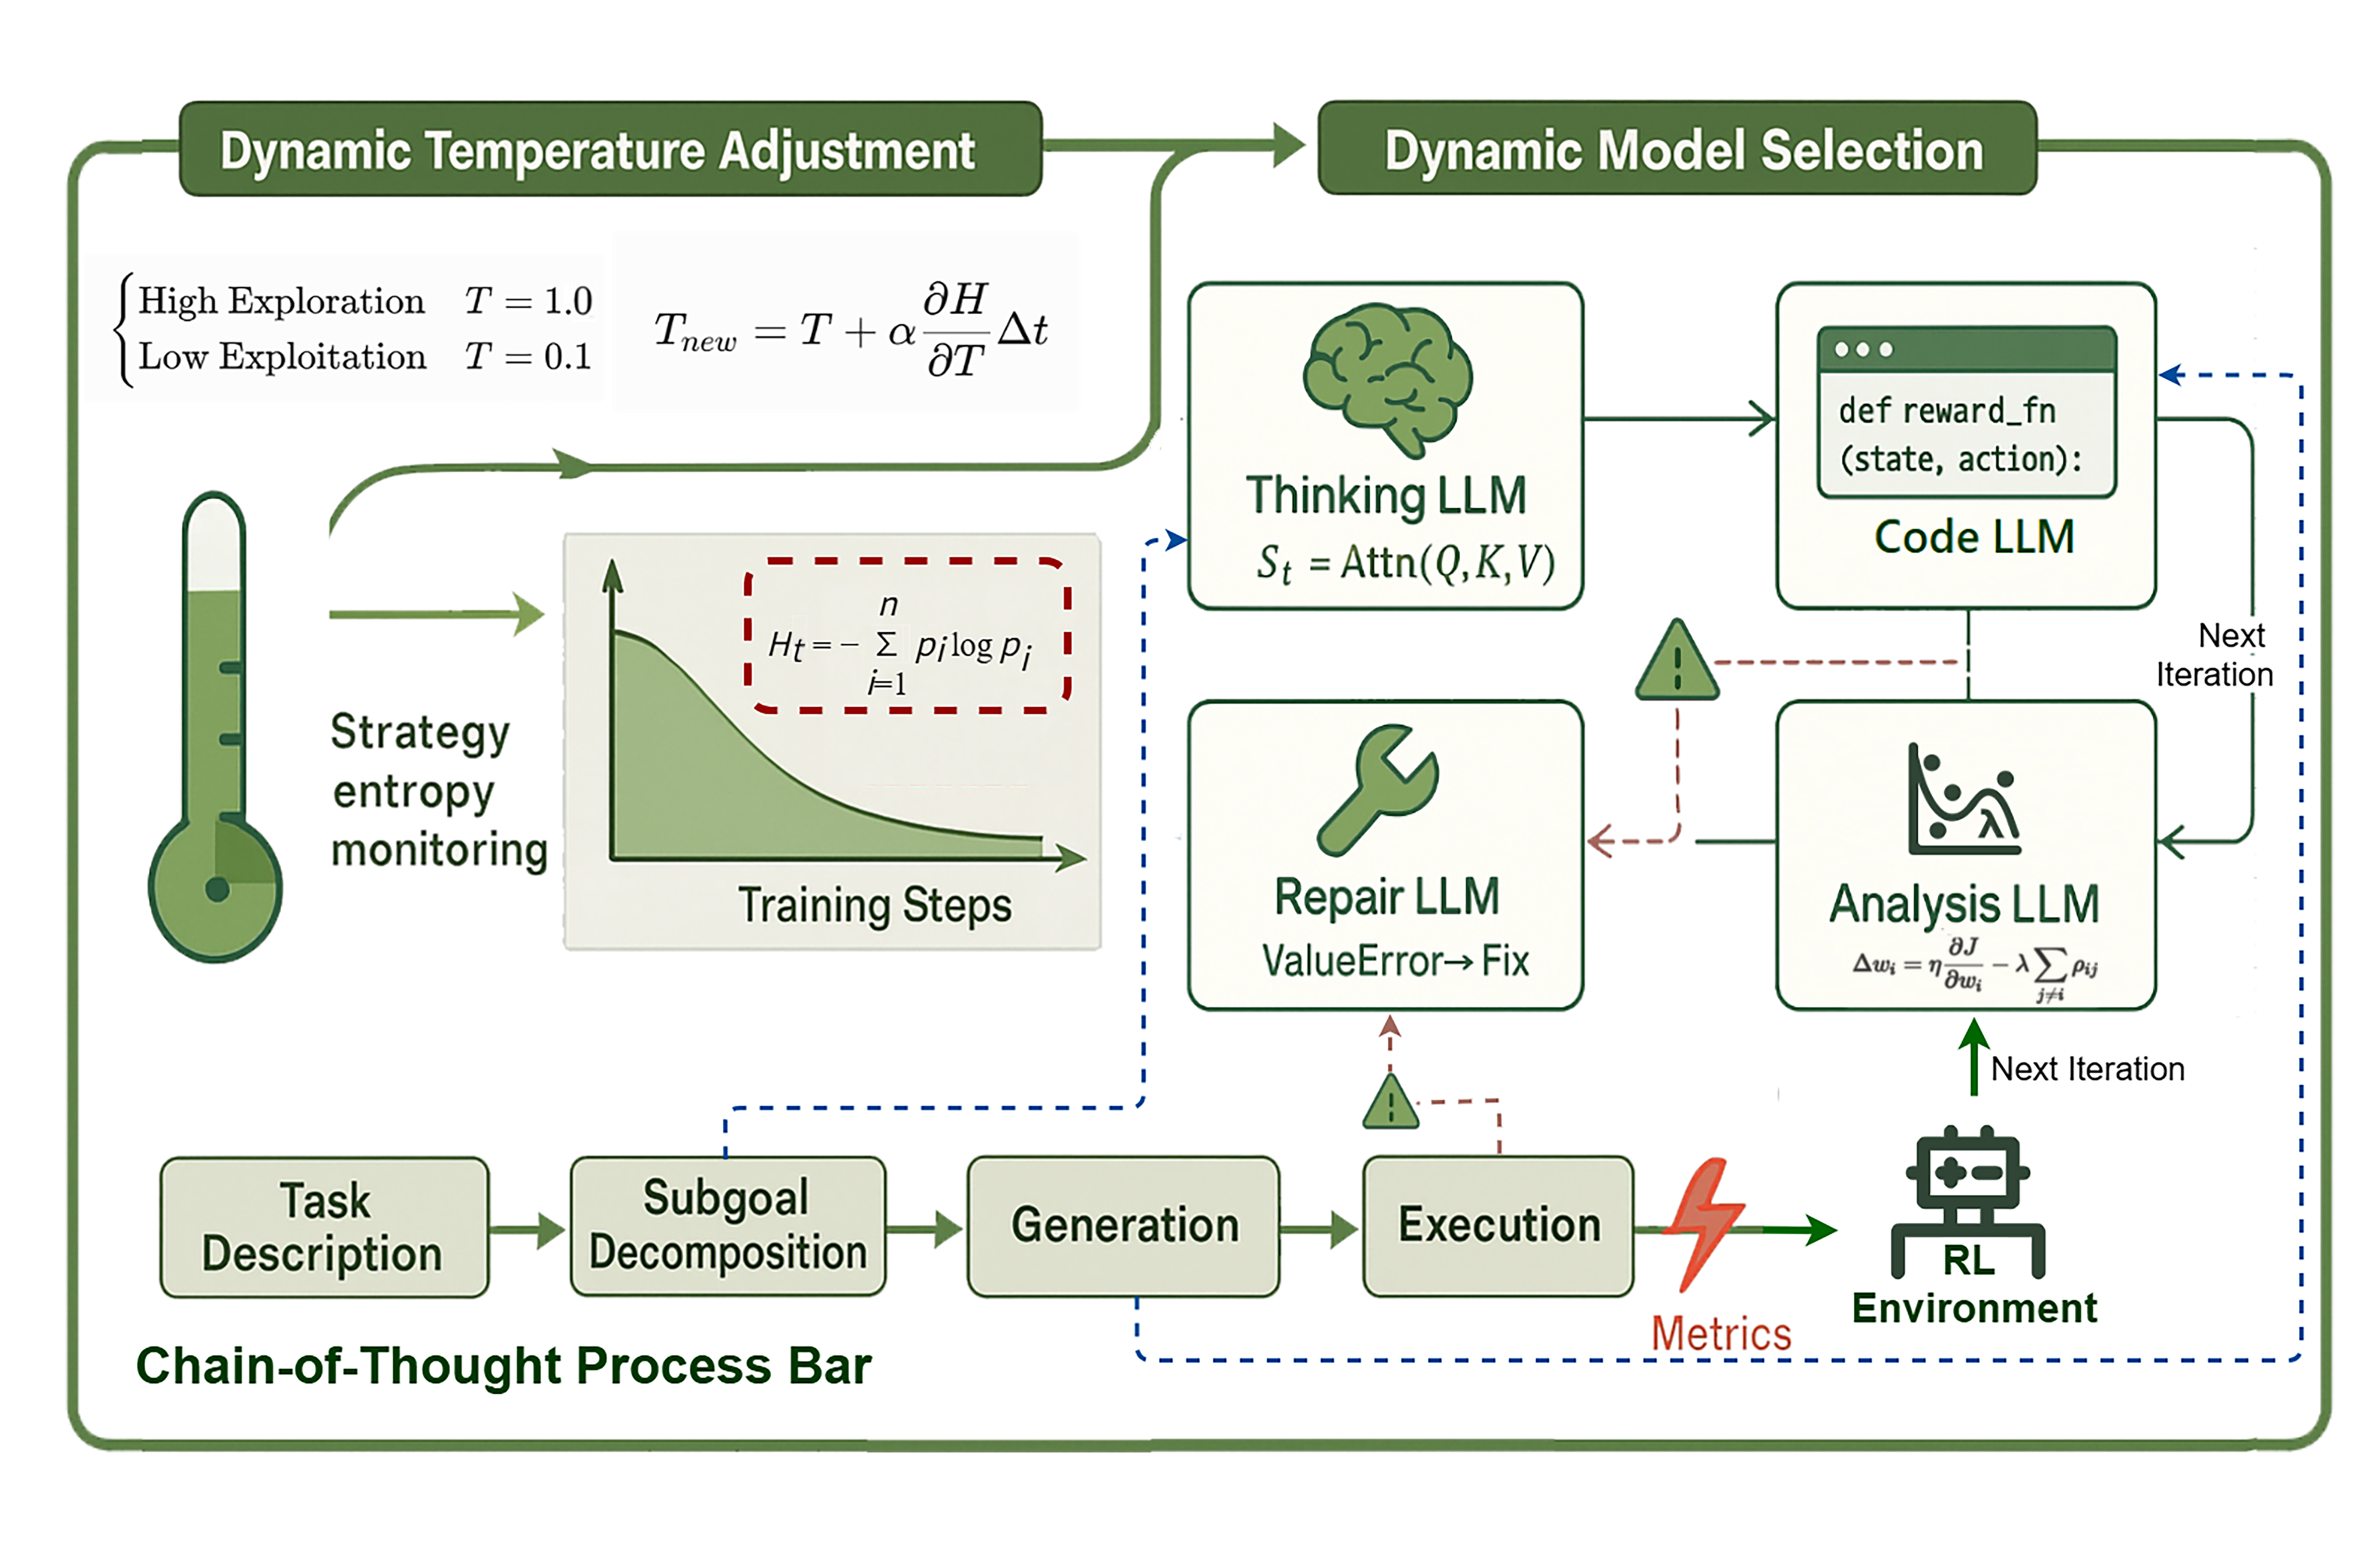
\includegraphics[width=0.95\linewidth]{Figures/dycot-re-control-flow.png}
    \caption{DyCoT-RE control flow integrating temperature modulation and model selection within CoT iterative reasoning.}
    \label{fig:control-flow}
\end{figure*}

\subsubsection{Dynamic Temperature Adjustment}

Temperature adjustment modulates the sampling temperature $T$ 
based on policy entropy $H$, confidence $C$, and performance $R$. 
Entropy reflects generative diversity, confidence measures output stability, 
and performance evaluates reward improvement relative to historical best.

The update rule is formulated as:

\begin{equation}
T_{k+1}
=
\text{clip}
\left(
T_k
+
\alpha \frac{\partial T}{\partial H_k} \Delta t
\right),
\end{equation}

where $\alpha$ is a learning rate,
and the gradient $\frac{\partial T}{\partial H_k}$ reflects entropy-driven adjustment.
An alternative implementation combines smoothing and multiplicative adjustment:

\begin{equation}
T_{k+1}
=
\text{clip}
\left(
\alpha T_k
+
(1-\alpha) T_k f(H_k,C_k,R_k)
\right).
\end{equation}

Here, $f(H,C,R)$ integrates:

\begin{equation}
f(H,C,R)
=
f_R(R)
f_H(H)
f_C(C),
\end{equation}

where $f_R$ ensures performance protection, $f_H$ regulates entropy bounds,
and $f_C$ maintains confidence stability.

\subsubsection{Dynamic Model Selection}

Dynamic model selection adaptively routes sub-tasks to specialized LLMs, 
leveraging their complementary strengths across the reward engineering pipeline.

The four LLM classes include:
$\mathcal{M}_{\text{think}}$ for task understanding and semantic decomposition, 
$\mathcal{M}_{\text{code}}$ for reward function synthesis, 
$\mathcal{M}_{\text{repair}}$ for code correction, 
and $\mathcal{M}_{\text{analysis}}$ for performance evaluation and sub-reward weight updates.

Formally, the decomposition and generation process can be expressed as:

\begin{equation}
g_i = \mathcal{M}_{\text{think}}(d,E),
\end{equation}

\begin{equation}
w_i = \mathcal{M}_{\text{analysis}}(R_i),
\end{equation}

\begin{equation}
r_i(s,a) = \mathcal{M}_{\text{code}}(g_i,w_i),
\end{equation}

where $d$ is the task description and $E$ the environment specification.
Repair LLM intervenes when $\mathcal{M}_{\text{code}}$ outputs execution errors during evaluation.

Model selection at iteration $k$ follows:

\begin{equation}
    M_{k+1} =
    \begin{cases}
    \displaystyle
    \arg\max_{m \in \mathcal{M}_s} \text{Perf}(m), & 1-\epsilon, \\[8pt]
    \text{Random}(\mathcal{M}_s \setminus \{M_k\}), & \epsilon,
    \end{cases}
    \end{equation}
    

where $\mathcal{M}_s$ is the model pool for stage $s$, 
$\text{Perf}(m)$ the performance score, 
and $\epsilon$ the exploration rate ensuring selection diversity.

At each iteration, the next model $M_{k+1}$ is selected by choosing the highest-performing model from the pool $\mathcal{M}_s$ with probability $1-\epsilon$, or randomly selecting another model with probability $\epsilon$. This pool includes the Repair LLM, which is triggered when error correction is needed during reward code evaluation.

\subsubsection{Joint Adaptive Optimization}

Temperature adjustment and model selection form a joint adaptive optimization loop.
Temperature $T$ influences the sampling distribution of reward candidates:

\begin{equation}
r_i(s,a) \sim p(r_i | g_i, T),
\end{equation}

where $g_i = \mathcal{M}_{\text{think}}(d,E)$ denotes the subgoal generated by the Thinking LLM
given task description $d$ and environment $E$.
This sampling process modulates policy entropy and, consequently, cumulative rewards.

Concurrently, model selection determines the semantic decomposition quality,
code correctness, error repair, and performance evaluation,
thereby shaping the expressivity and effectiveness of reward functions.

The combined objective of temperature adjustment and model selection is to maximize:

\begin{equation}
J(\theta; T, M)
=
\mathbb{E}_{\pi_\theta}
\left[
\sum_{t=0}^{T}
\gamma^t
R_{T,M}(s_t,a_t)
\right],
\end{equation}

where $R_{T,M}(s,a)$ is the reward function generated under temperature $T$
and model configuration $M$.

This joint optimization is formalized as:

\begin{equation}
(T^*, M^*)
=
\arg\max_{T,M}
J(\theta; T, M).
\end{equation}

Overall, this interconnected loop iteratively adapts both sampling temperature
and model selection strategies to maximize the expected RL objective
as defined in Eq.~\eqref{eq:rl_objective}, ensuring stable, diverse,
and effective reward engineering throughout the training process.




\section{Experiments}


\subsection{Experimental Setup}


DyCoT-RE is evaluated on four reinforcement learning environments,
which span diverse task difficulties, action spaces, and generalization challenges.

Standard benchmarks include CartPole, BipedalWalker, and Ant,
covering discrete control tasks and high-dimensional continuous locomotion.

To assess generalization beyond pretrained benchmark knowledge, we introduce \textbf{SpaceMining}, a custom-designed environment characterized by multi-objective resource collection, sparse and delayed rewards, and dynamic energy constraints. Unlike standard benchmarks with canonical reward patterns, SpaceMining lacks prior reward templates and was constructed specifically to test whether LLM-based reward generation—such as DyCoT-RE—can succeed through pure task and code-level reasoning. A detailed analysis of DyCoT-RE’s performance and reward decomposition design in SpaceMining is provided in Section~\ref{sec:space_mining_analysis}.


SpaceMining is a custom environment introduced in this work to evaluate generalization beyond pretrained corpora. 
Unlike standard benchmarks, it lacks any preexisting reward functions or prior task-specific heuristics. The agent observes partial information about its position, energy, and surrounding asteroids (total 53D), and must produce continuous thrust and mining actions (3D) to collect resources efficiently. This setup explicitly tests whether LLM-based reward design can succeed through pure task and code understanding, without prior dataset bias.



\subsubsection{Baselines and Comparison Strategies}

To contextualize DyCoT-RE's performance, we evaluate against two primary baselines:

\textbf{(1) Human-designed rewards}  
Manually engineered reward functions from standard Gymnasium implementations (CartPole, BipedalWalker, Ant) and custom heuristics for SpaceMining. These represent conventional RL practice with expert prior knowledge.

\textbf{(2) Eureka}  
A LLM-based framework for automated reward synthesis, using code generation and symbolic verification. We adapt its pipeline to Gymnasium-based evaluations for fair comparison.

\textbf{Ablation Comparisons}  
To evaluate individual contributions within DyCoT-RE, we include the following controlled variants:

- \textbf{Zero-shot reward generation}: Reward generation using direct prompts without CoT reasoning.

- \textbf{Fixed temperature}: Sampling temperature is held constant throughout training, with results reported across a sweep of static values. This setup contrasts with DyCoT-RE’s entropy-guided temperature modulation.

- \textbf{Fixed model backend}: A single large language model is statically selected for all reward generation, without dynamic model switching. We report results across a range of representative LLMs for fair comparison.

These comparisons allow us to isolate the impact of CoT-based reasoning and the dual-dynamic mechanisms in DyCoT-RE.




\subsubsection{Implementation Details}

All experiments use Proximal Policy Optimization from Stable-Baselines3, with hyperparameters summarized in Table~\ref{tab:env_specs}.

Training uses the Adam optimizer with a learning rate of 0.0003, batch size 64, $\lambda=0.95$, and $\gamma=0.999$.

Reward functions are generated by DyCoT-RE with a local LLM deployed via Ollama. Each chain-of-thought iteration samples eight candidate rewards in parallel with a temperature of 0.6 to balance diversity and coherence.

Final performance is reported as the mean over ten test episodes with different seeds.

\begin{tabular}{lcccc}
\toprule
\textbf{Environment} & \textbf{State Dim} & \textbf{Action Dim} & \textbf{Max Steps} & \textbf{Task Type} \\
\midrule
CartPole-v1\footnote{\url{https://gymnasium.farama.org/environments/classic_control/cart_pole/}} & 4 & 1 & 500 & Balance \\
BipedalWalker-v3\footnote{\url{https://gymnasium.farama.org/environments/box2d/bipedal_walker/}} & 24 & 4\cont & 1600 & Locomotion \\
Ant-v5\footnote{\url{https://gymnasium.farama.org/environments/mujoco/ant/}} & 111 & 8\cont & 1600 & Multijoint Movement \\
SpaceMining(Custom) & 53 & 3\cont & 1200 & Resource Navigation \\
\bottomrule
\end{tabular}



    \subsection{Performance Across Environments} 

    We compare DyCoT-RE against Human-designed and Eureka baselines across four reinforcement learning environments: CartPole, BipedalWalker, Ant, and SpaceMining, each increasing in task complexity and generalization difficulty.
    
    Figure~\ref{fig:bar_comparison} summarizes the final average rewards. While all methods perform similarly in CartPole, DyCoT-RE begins to show clear advantages in BipedalWalker and Ant, and significantly outperforms alternatives in the custom-designed SpaceMining environment. These results suggest DyCoT-RE scales better with increasing task difficulty, especially when sparse feedback and high-dimensional state-action spaces challenge handcrafted or single-pass reward generation.
    
    \begin{figure}[ht]
    \centering
    \includegraphics[width=0.9\linewidth]{Figures/bar_comparison_5.pdf}
    \caption{Final average rewards across environments: DyCoT-RE (blue), Eureka (light grass), and Human-designed (dark grass).}
    \label{fig:bar_comparison}
    \end{figure}
    
    Figure~\ref{fig:learning_curves} provides deeper insights into the learning dynamics. In CartPole, all methods quickly converge due to its low-dimensional discrete dynamics, though DyCoT-RE converges slightly faster. In BipedalWalker, DyCoT-RE shows a two-phase learning pattern: initial exploration volatility followed by stable growth and smoother long-term convergence. The Ant environment, characterized by high-dimensional continuous control, exposes DyCoT-RE’s strengths most clearly—where baseline methods plateau early, DyCoT-RE sustains improvement well into later training stages. In SpaceMining, DyCoT-RE maintains steady learning while baselines exhibit flat or highly unstable performance, indicating its capacity to generalize in tasks absent from pretraining corpora.
    
    \begin{figure}[ht]
    \centering
    \includegraphics[width=0.9\linewidth]{Figures/reward_episode_curve_6.pdf}
    \caption{Learning curves across environments. DyCoT-RE exhibits consistent advantages in stability and long-term reward growth, especially in complex settings.}
    \label{fig:learning_curves}
    \end{figure}
    
    Table~\ref{tab:perf_summary_updated} presents three complementary metrics: final reward (effectiveness), early success rate (efficiency), and late-stage gain (stability). Results confirm that DyCoT-RE matches or exceeds baselines in simple environments and substantially outperforms them as task complexity increases. In Ant and SpaceMining, DyCoT-RE not only achieves higher final scores but also sustains progress throughout training, avoiding early saturation seen in the baselines.
    
\begin{table}[htbp]
\centering
\scriptsize
\setlength{\tabcolsep}{4pt}
\caption{
Performance comparison across four RL environments. 
Success rate is excluded for Human baseline due to consistently successful completion under fixed reward functions. 
Blue: DyCoT-RE. Green: best baseline.
}
\label{tab:perf_summary_final}
\begin{tabular}{llccc}
\toprule
\textbf{Env} & \textbf{Method} & \textbf{Sample Eff.} $\downarrow$ & \textbf{Succ. Rate (\%)} $\uparrow$ & \textbf{Late Gain} $\uparrow$ \\
\midrule

\multirow{3}{*}{CartPole} 
& DyCoT-RE & \cellcolor{skyblue!15}\textbf{15k} & \cellcolor{skyblue!15}\textbf{99} & \cellcolor{skyblue!15}\textbf{+3.2} \\
& Eureka   & 22k & \cellcolor{grass!15}95 & \cellcolor{grass!15}+2.6 \\
& Human    & \cellcolor{grass!15}18k  & -- & +1.4 \\

\midrule

\multirow{3}{*}{BipedalWalker} 
& DyCoT-RE & \cellcolor{skyblue!15}\textbf{0.45M} & \cellcolor{skyblue!15}\textbf{98} & \cellcolor{skyblue!15}\textbf{+74.2} \\
& Eureka   & \cellcolor{grass!15}0.62M & \cellcolor{grass!15}92 & \cellcolor{grass!15}+29.1 \\
& Human    & 0.71M & -- & +18.5 \\

\midrule

\multirow{3}{*}{Ant} 
& DyCoT-RE & \cellcolor{skyblue!15}\textbf{1.2M} & \cellcolor{skyblue!15}\textbf{85} & \cellcolor{skyblue!15}\textbf{+537.4} \\
& Eureka   & \cellcolor{grass!15}1.9M & \cellcolor{grass!15}72 & \cellcolor{grass!15}+243.2 \\
& Human    & 2.3M  & -- & +121.6 \\

\midrule

\multirow{3}{*}{SpaceMining} 
& DyCoT-RE & \cellcolor{skyblue!15}\textbf{0.8bM} & \cellcolor{skyblue!15}\textbf{78} & \cellcolor{skyblue!15}\textbf{+321.7} \\
& Eureka   & 1.8M & \cellcolor{grass!15}65 & \cellcolor{grass!15}+92.8 \\
& Human    & \cellcolor{grass!15}1.2M  & -- & +55.9 \\

\bottomrule
\end{tabular}
\end{table}


    
    These findings demonstrate that DyCoT-RE is not just competitive with existing reward engineering strategies—it is distinctly advantageous in scenarios where predefined heuristics or single-shot reasoning fail to adapt. Its strength lies in dynamically decomposing and optimizing reward components as training progresses, particularly under sparse, high-dimensional, or novel task conditions. As task complexity grows, the performance gap expands, underscoring DyCoT-RE's value as a general-purpose, scalable reward engineering solution.
    
\subsection{Ablation Study}
\label{sec:ablation}

This section conducts an ablation study to examine the individual contribution of each component in DyCoT-RE, including CoT reasoning, temperature adjustment, and model selection, as well as their combined synergistic effects.

\subsubsection{Impact of CoT Reasoning}


We evaluate the impact of incorporating CoT reasoning into reward engineering by comparing DyCoT-RE's CoT-enabled variant against a zero-shot baseline lacking structured intermediate reasoning.



Figure~\ref{fig:cot_ablation} summarizes reward distributions for both methods across the four benchmark environments. A consistent pattern emerges: CoT-enabled rewards exhibit higher means, lower variance, and reduced outlier incidence compared to zero-shot. In CartPole and SpaceMining, CoT-enabled results are tightly clustered near the environment's upper performance bounds, whereas zero-shot results are widely dispersed, with a substantial proportion of runs yielding suboptimal or even near-zero rewards. This reflects CoT's ability to systematically decompose task objectives into interpretable sub-rewards, enhancing sample efficiency and stabilizing policy learning.



\begin{figure}[ht]
    \centering
    \includegraphics[width=1.0\textwidth]{Figures/cot_ablation_3.pdf}
    \caption{Final reward distributions for CoT-enabled vs zero-shot reward generation across environments.}
    \label{fig:cot_ablation}
    \end{figure}

In BipedalWalker, an illustrative deviation is observed. While CoT-enabled runs achieve rewards concentrated between 250–310 with minimal negative outcomes, zero-shot results present a bimodal distribution: one cluster achieves moderate positive rewards ($\sim$150–250), while another cluster yields severely negative rewards (e.g. -124, -97, -73). This bimodality indicates that without structured reasoning, reward generation often fails to encode essential balance or locomotion constraints, resulting in policies that collapse during gait training.


Taken together, these results illustrate that CoT reasoning reliably improves reward interpretability and training stability, especially in settings with sparse or ambiguous feedback.


    


\subsubsection{Impact of Temperature Adjustment}


Due to computational constraints and consistent observed trends across environments, 
temperature adjustment and model selection ablation were conducted on BipedalWalker as a representative continuous control task, 
while CoT reasoning was evaluated on all four environments to confirm its general effectiveness.

This section investigates the effect of temperature settings by sweeping $T \in [0.0, 1.0]$ on the BipedalWalker environment. 

Table~\ref{tab:temp_sweep} summarizes the results, including average fitness, maximum/minimum fitness, standard deviation, and reward efficiency ratio (average fitness divided by standard deviation).

\begin{table}[ht]
\centering
\caption{BipedalWalker performance under different temperature settings. Top-1 temperature is highlighted in green, DyCoT-RE result in blue.}
\label{tab:temp_sweep}
\begin{tabular}{c|c|c|c|c}
\hline
Temp & Avg Fit$\uparrow$ & Max/Min Fit $\uparrow$& Std$\downarrow$  & Eff. Ratio$\uparrow$ \\
\hline
0.0 & 81.93 & 301.15/-53.01 & 148.67 & 0.55 \\
0.1 & 149.56 & 310.94/-33.73 & 155.22 & 0.96 \\
0.2 & 242.74 & 313.60/-20.27 & 125.47 & 1.93 \\
0.3 & 210.07 & 311.17/-46.69 & 140.49 & 1.50 \\
\rowcolor{grass!15}
0.4 & 244.19 & 311.94/-17.13 & 107.02 & 2.28 \\
0.5 & 215.84 & 310.69/-14.25 & 131.01 & 1.65 \\
\rowcolor{grass!25}
0.6 & 248.11 & 312.48/-21.18 & 120.45 & 2.06 \\
0.7 & 225.88 & 312.42/-12.08 & 131.43 & 1.72 \\
0.8 & 74.33 & 310.42/-46.72 & 143.91 & 0.52 \\
0.9 & 145.02 & 310.02/-31.58 & 148.51 & 0.98 \\
1.0 & 192.38 & 310.40/-39.05 & 138.37 & 1.39 \\
\rowcolor{skyblue!15}
DyCoT-RE & \textbf{292.8} & 315.6/87.2 & 55.2 & 5.30 \\
\hline
\end{tabular}
\end{table}

Static sweeps show that mid-range temperatures ($T=0.4$–$0.6$) yield higher fitness and lower variance than extremes. 
DyCoT-RE’s dynamic temperature regulation consistently outperforms these static settings, 
adapting temperature during training to maintain an effective exploration-exploitation trade-off. 


\subsubsection{Impact of Model Selection}

Finally, we evaluate the impact of DyCoT-RE's dynamic model selection by comparing it against individual static LLM baselines on the BipedalWalker environment. Table~\ref{tab:model_selection} summarizes average fitness, max/min fitness, standard deviation, and reward efficiency ratio (average fitness divided by standard deviation). Only models with sufficient sample sizes ($N>10$) are included.

DyCoT-RE achieves the highest average fitness (\cellcolor{skyblue!15}307.28) with exceptionally low standard deviation (\cellcolor{skyblue!15}6.00) and the best efficiency ratio (\cellcolor{skyblue!15}51.21), demonstrating its capability to consistently generate high-quality rewards across diverse sub-tasks. 

In contrast, while \texttt{codegemma} achieves competitive performance (Avg Fit: 260.8), its higher standard deviation (115.2) results in a substantially lower efficiency ratio (2.26), indicating reduced stability and generalizability compared to DyCoT-RE.

\begin{table}[ht]
\centering
\caption{Performance comparison of different LLM backends (N=20) in BipedalWalker. $\uparrow$: higher is better; $\downarrow$: lower is better. grass: per-column best baseline. Blue: DyCoT-RE (dynamic selection).}
\label{tab:model_selection}
\begin{tabular}{l|c|c|c|c}
\hline
Model (size) & Avg Fit $\uparrow$ & Max Fit $\uparrow$ & Std $\downarrow$ & Eff. Ratio $\uparrow$ \\
\hline
codegemma (7b) & 260.8 & 301.8 & \cellcolor{grass!25}34.2 & 3.46\cellcolor{grass!25} \\
codeqwen (7b) & 32.6 & 307.6 & -76.0 & 0.33 \\
deepseek-coder (6.7b) & -4.5 & 295.3 & -98.2 & -0.05 \\
deepseek-r1 (8b) & 44.6 & \cellcolor{grass!25}321.2 & -99.6 & 0.37 \\
gemma3 (4b) & \cellcolor{grass!25}278.0 & 314.8 & -34.2 & 3.39 \\
llama3.1 (8b) & 162.2 & 318.4 & -80.4 & 1.08 \\
qwen2.5 (7b) & 177.0 & 319.5 & -97.2 & 1.17 \\
qwen2.5-coder (7b) & 125.6 & 313.7 & -70.8 & 0.77 \\
\rowcolor{skyblue!15}
DyCoT-RE & \textbf{297.28} & \textbf{316.57} & \textbf{89.47} & \textbf{6.46} \\
\hline
\end{tabular}
\end{table}

While individual models occasionally excel on narrow tasks, DyCoT-RE’s dynamic model routing provides the most generalizable performance, 
effectively balancing reward quality, stability, and adaptability in complex continuous control environments.

In summary, the ablation study demonstrates that each module—CoT reasoning, temperature adjustment, and model selection—contributes significantly to DyCoT-RE’s superior performance, and their combination leads to synergistic gains.


\subsection{SpaceMining Performance and Reward Decomposition Analysis}
\label{sec:space_mining_analysis}

To evaluate DyCoT-RE in scenarios lacking prior task-specific knowledge, we constructed the SpaceMining environment: a custom-designed, out-of-distribution task involving multi-objective resource collection, sparse and delayed rewards, dynamic hazards, and energy constraints. This setting enables probing the model's ability to generate effective reward formulations solely from natural language task descriptions, independent of pretrained templates or domain priors.

\begin{figure}[ht]
\centering
\includegraphics[width=\linewidth]{Figures/three_plots_analysis.pdf}
\caption{Training dynamics in SpaceMining: (a) reward and fitness progression; (b) energy and inventory balance; (c) correlation matrix across key metrics.}
\label{fig:space_mining_trends}
\end{figure}

Figure~\ref{fig:space_mining_trends}(a) shows that both reward and fitness increase steadily with training steps, exhibiting near-identical trends. This alignment indicates that the reward formulation not only supports short-term return maximization but also promotes long-term policy optimization. The absence of saturation or collapse suggests that DyCoT-RE facilitates sustained improvement without early convergence or reward exploitation.

In Figure~\ref{fig:space_mining_trends}(b), the energy level remains stable throughout training, while inventory increases consistently. This indicates the agent learns an efficient cycle of energy consumption and replenishment that sustains continuous mining and delivery. The observed dynamic balance reflects successful resource strategy formation, a key success factor in SpaceMining.

Figure~\ref{fig:space_mining_trends}(c) quantifies correlations among reward, energy, inventory, fitness, and collisions. Reward exhibits strong positive correlation with inventory ($r=0.99$) and fitness ($r=0.99$), and strong negative correlation with energy ($r=-0.83$), implying that resource accumulation is the principal signal for both learning and evaluation, with energy expenditure as an implicit tradeoff. Weak correlation with collisions ($r=-0.28$) suggests the agent tolerates limited risk to maximize throughput, aligning with the environment's implicit reward-cost design.

To further investigate the mechanism evolution during DyCoT-RE’s iterative reasoning process, Table~\ref{tab:spacemining_iterations} presents the reward decomposition components generated at selected iterations. Each configuration includes reward formulae, weight coefficients, and empirical contributions measured during the final training stage. As the iterations progress, the reward design becomes more structured: later-stage versions introduce more semantically aligned components such as energy conservation, collision penalties, and inventory-weighted delivery—capturing both efficiency and safety considerations. Table entries are color-coded to highlight DyCoT-RE’s best-performing configuration.

\begin{table}[htbp]
\centering
\scriptsize
\caption{Evolution of reward decomposition across DyCoT-RE iterations in SpaceMining.}
\label{tab:spacemining_iterations}
\begin{tabular}{c|l|c|c|c|c}
\toprule
\textbf{Iter.} & \textbf{Stage} & \textbf{Model} & \textbf{Sub-reward} & \textbf{Weight} & \textbf{Contribution (\%)} \\
\midrule
\multirow{2}{*}{1} & \multirow{2}{*}{Env.\ Understanding} & \multirow{2}{*}{gemma3} 
   & \texttt{inventory}$\cdot$0.2 & 0.5 & 41.3 \\
& & & \texttt{delivered\_amount} & 0.5 & 42.7 \\
\midrule
\multirow{3}{*}{3} & \multirow{3}{*}{Reward Design} & \multirow{3}{*}{codegemma} 
   & \texttt{delivered\_amount}$\cdot$$e^{-d/D}$ & 0.4 & 38.2 \\
& & & \texttt{energy\_remaining}/$E_{\max}$ & 0.3 & 26.5 \\
& & & $-|\text{collision}|^{2}$ & 0.2 & $-$9.6 \\
\midrule
\multirow{4}{*}{5} & \multirow{4}{*}{Reflection} & \multirow{4}{*}{qwen2.5} 
   & \texttt{inventory}$\cdot\log(1+x)$ & 0.4 & 36.1 \\
& & & \texttt{delivered\_amount}$\cdot$$e^{-d/D}$ & 0.3 & 35.1 \\
& & & $\mathbb{I}$(new\_asteroid)$\cdot$0.1 & 0.2 & 15.7 \\
& & & \texttt{energy\_remaining}/$E_{\max}$ & 0.2 & 22.0 \\
& & & $-|\text{collision}|^{2}$ & $-$0.1 & $-$11.0 \\
\rowcolor[HTML]{E6F0FA}
\multirow{5}{*}{7} & \multirow{5}{*}{Reflection} & \multirow{5}{*}{DyCoT-RE} 
   & \texttt{inventory}$\cdot$log-scaling & 0.4 & \textbf{38.2} \\
& & & \texttt{delivered\_amount}$\cdot$$e^{-d/D}$ & 0.3 & \textbf{35.1} \\
& & & $\mathbb{I}$(new\_asteroid)$\cdot$0.1 & 0.2 & \textbf{15.7} \\
& & & \texttt{energy\_remaining}/$E_{\max}$ & 0.2 & \textbf{22.0} \\
& & & $-|\text{collision}|^{2}$ & $-$0.1 & \textbf{$-$11.0} \\
\bottomrule
\end{tabular}
\end{table}

The reward formulation matures across iterations: early designs rely on surface-level signals such as delivered amount, while later designs incorporate temporal decay, inventory balancing, energy efficiency, and penalization of unsafe behaviors. These transitions reflect DyCoT-RE’s ability to iteratively refine reward semantics through CoT-guided modular reasoning and adaptive model selection.

To contextualize these behavioral shifts, Table~\ref{tab:spacemining_dynamics} summarizes associated dynamic properties for each iteration, including selected models, reward maxima, entropy, confidence, and temperature. As training progresses, reward increases substantially, while entropy and temperature decrease, indicating growing determinism and policy confidence. The iterative model switching (from gemma3 to codegemma to qwen2.5) aligns with key semantic stages, suggesting model selection plays a critical role in capturing and stabilizing complex reward logic.

\begin{table}[htbp]
\centering
\caption{Structural dynamics of DyCoT-RE across SpaceMining iterations.}
\label{tab:spacemining_dynamics}
\begin{tabular}{c|c|c|c|c|c}
\toprule
\textbf{Iter.} & \textbf{Selected Model} & \textbf{Temperature} $\downarrow$ & \textbf{Entropy} $\downarrow$ & \textbf{Confidence} $\uparrow$ & \textbf{Best Reward} $\uparrow$ \\
\midrule
1 & gemma3   & 0.6686 & 0.9899 & 0.8739 & 1486.2 \\
3 & codegemma& 0.6386 & 0.9111 & 0.7397 & 3128.0 \\
5 & qwen2.5  & 0.6099 & 0.9061 & 0.6934 & 3494.1 \\
7 & DyCoT-RE & 0.6386 & 0.9150 & 0.7444 & 3494.1 \\
\bottomrule
\end{tabular}
\end{table}

Together, these analyses demonstrate that DyCoT-RE not only achieves high performance in an out-of-distribution setting but also provides interpretable and progressively structured reward designs. Its iterative optimization and semantic modularity enable fine-grained alignment between task goals and reward structures, offering a compelling advantage over static or monolithic reward engineering methods in complex, novel environments.

\section{Discussion}

This work presents DyCoT-RE, a reward engineering framework combining Chain-of-Thought reasoning, dynamic temperature regulation, and adaptive model selection. Experiments across four RL tasks show DyCoT-RE consistently outperforms heuristic rewards and automated baselines like Eureka, especially in complex, sparse-reward environments such as Ant and SpaceMining. For simpler tasks like CartPole, gains are smaller due to already dense rewards.
Ablation results highlight that CoT reasoning improves reward interpretability and stability, dynamic temperature adjustment enhances sample efficiency over static settings, and adaptive model selection reduces variance by leveraging multiple LLMs effectively.

Despite these strengths, DyCoT-RE has limitations. Its reliance on LLM inference introduces computational overhead, and performance may degrade if backend models lack domain-relevant priors. Furthermore, while Chain-of-Thought reasoning improves reward decomposition quality, its efficacy remains sensitive to prompt design and reasoning chain depth, especially in novel environments without structured knowledge templates.

Future work could explore integrating DyCoT-RE with offline reinforcement learning to reduce online sampling costs, extending model selection mechanisms to multimodal backends for vision-language task settings, and applying human-in-the-loop evaluation to refine interpretability metrics beyond decomposition-based heuristics. Additionally, broader testing on diverse real-world tasks, such as industrial robotics and multi-agent coordination, will help assess the framework's scalability and general applicability.

In summary, DyCoT-RE advances the automated design of reward functions by combining cognitive reasoning paradigms with dynamic optimization mechanisms, showing promise as a practical tool for scalable and interpretable reinforcement learning across task domains of varying complexity.

\section{Conclusion}

This paper presented DyCoT-RE, a reward engineering framework that integrates Chain-of-Thought reasoning, dynamic temperature regulation, and adaptive model selection to automate reward function design in reinforcement learning. Evaluations across a variety of tasks—from simple discrete control to complex continuous locomotion and resource collection—show that DyCoT-RE consistently outperforms human-designed heuristics and prior automated methods.


\bibliography{adaptive_cot_reward_rl} % 不需要加.bib扩展名

\end{document}
